\documentclass{article}
\usepackage[utf8]{inputenc}
\usepackage[english]{babel}
\usepackage{amsmath}
\usepackage[]{amsthm} %lets us use \begin{proof}
\usepackage[]{amssymb} %gives us the character \varnothing
%\usepackage[utf8]{vietnam}
\usepackage{indentfirst}
\usepackage{CJKutf8}
\usepackage{enumitem}
\usepackage{tikz}
\usetikzlibrary{matrix}
\usepackage{graphicx}
\newcounter{rown}
\newcounter{rownn}
\newcounter{rownm}
\newcommand{\row}[2]{\stepcounter{rown}\arabic{rown} & #1 & #2 \\}
\newcommand{\roww}[2]{\stepcounter{rownn}\arabic{rownn} & #1 & #2 \\}
\newcommand{\rowq}[2]{\stepcounter{rownm}\arabic{rownm} & #1 & #2 \\}
\title{Homework 1B}
\author{Nguyen Tuan Anh - ID: 2252038 - CN01}
\begin{document}
\maketitle
\section*{Section 1.4}
\subsection*{Exercise 9}
Let P(x) be the statement “x can speak Russian” and let Q(x) be the statement “x knows the computer language C++.” Express each of these sentences in terms of P(x), Q(x), quantifiers, and logical connectives. The domain for quantifiers consists of all students at your school.
\begin{enumerate} [label = (\alph*)]
    \item There is a student at your school who can speak Russian and who knows C++.
    \item There is a student at your school who can speak Russian but who doesn’t know C++.
    \item Every student at your school either can speak Russian or knows C++.
    \item No student at your school can speak Russian or knows C++.
\end{enumerate}

\subsubsection*{Solution}
We have that $P(x)$: "x can speak Russian" and $Q(x)$: "x knows the computer language C++".
\begin{enumerate} [label = (\alph*)]
    \item $\exists x(P(x) \land Q(x))$
    \item $\exists x(P(x) \land \lnot Q(x))$
    \item $\forall x (P(x) \lor Q(x))$
    \item $\forall x \lnot(P(x) \lor Q(x))$
\end{enumerate}

\subsection*{Exercise 10}
Let C(x) be the statement “x has a cat,” let D(x) be the statement “x has a dog,” and let F(x) be the statement “x has a ferret.” Express each of these statements in terms of C(x), D(x), F(x), quantifiers, and logical connectives. Let the domain consist of all students in your class.
\begin{enumerate} [label = (\alph*)]
    \item A student in your class has a cat, a dog, and a ferret.
    \item All students in your class have a cat, a dog, or a ferret.
    \item Some student in your class has a cat and a ferret, but not a dog.
    \item No student in your class has a cat, a dog, and a ferret.
    \item For each of the three animals, cats, dogs, and ferrets, there is a student in your class who has this animal as a pet.
\end{enumerate}
\subsubsection*{Solution}
We have that $C(x)$: "x has a cat", $D(x)$: "x has a dog", $F(x)$: "x has a ferret".
\begin{enumerate} [label = (\alph*)]
    \item $\exists x(C(x) \land D(x) \land F(x))$
    \item $\forall x(C(x) \lor D(x) \lor F(x))$
    \item $\exists x(C(x) \land F(x) \land \lnot D(x))$
    \item $\forall x\lnot(C(x) \land D(x) \land F(x))$
    \item
          Because in this case, each animal will have a different owner and this statement will become true if all of the pets are all have their owners. Therefore, we have that:
          \begin{align}
              \exists xC(x) \land \exists yD(y) \land \exists zF(z) \nonumber
          \end{align}
\end{enumerate}
\subsection*{Exercise 33}
Express each of these statements using quantifiers. Then form the negation of the statement, so that no negation is to the left of a quantifier. Next, express the negation in simple English. (Do not simply use the phrase “It is not the case that.”)
\begin{enumerate} [label = (\alph*)]
    \item Some old dogs can learn new tricks.
    \item No rabbit knows calculus.
    \item Every bird can fly.
    \item There is no dog that can talk.
    \item There is no one in this class who knows French and Russian.
\end{enumerate}
\subsubsection*{Solution}
\begin{enumerate} [label = (\alph*)]
    \item Let's $P(x)$: "x can learn new tricks." and x will be "old dogs" $\rightarrow$ $\exists xP(x)$. In negation form, it will be: $\forall x\lnot P(x)$ and can be written as "No old dog can learn new tricks".
    \item Let's $Q(x)$: "x knows calculus" and x will be "rabbit" $\rightarrow$ $\forall x \lnot Q(x)$. In negation form, it will be: $\exists x Q(x)$ and can be written as "Some rabbits know calculus".
    \item Let's $D(x)$: "x can fly" and x will be "bird" $\rightarrow$ $\forall xD(x)$. In negation form, it will be: $\exists x\lnot D(x)$ and can be written as "Some birds can not fly".
    \item Let's $F(x)$: "x can talk" and x will be "dog" $\rightarrow$ $\forall x\lnot F(x)$. In negation form, it will be: $\forall xF(x)$ and can be written as "All dogs can talk".
    \item Let's $A(x)$: "x knows French", $B(x)$: "x knows Russian" and x will be "student" $\rightarrow$ $\forall x\lnot(A(x) \land B(x))$. In negation form, it will be $\exists x(A(x) \land B(x))$ and can be written as "There is a student who knows French and Russian".
\end{enumerate}

\subsection*{Exercise 34}
Express the negation of these propositions using quantifiers, and then express the negation in English.
\begin{enumerate} [label = (\alph*)]
    \item Some drivers do not obey the speed limit.
    \item All Swedish movies are serious.
    \item No one can keep a secret.
    \item There is someone in this class who does not have a good attitude.
\end{enumerate}
\subsubsection*{Solution}
\begin{enumerate} [label = (\alph*)]
    \item Let's $P(x)$: "x obeys the speed limit" and x is "driver" $\rightarrow \exists x\lnot P(x)$. In negation form, it will be $\forall xP(x)$ and can be translated to "All drivers obey the speed limit".
    \item Let's $Q(x)$: "x are serious" and x is "Swedish movies" $\rightarrow \forall xQ(x)$. In negation form, it will be $\exists x\lnot Q(x)$ and can be translated to "There is some Swedish movies are not serious".
    \item Let's $R(x)$: "x can keep a secret" and x is "people" $\rightarrow \forall x\lnot R(x)$. In negation form, it will be $\exists xR(x)$ and can be translated to "There is someone who can keep a secret".
    \item Let's $D(x)$: "x has a good attitude" and x is "student" and the domain of x will be the student in the class and the domain will be called $W$ $\rightarrow \exists x\in W\lnot D(x)$. In negation form, it will be $\forall x\notin WD(x)$ and can be translated to "All of the students who are not in this class have a good attitude".
\end{enumerate}

\subsection*{Exercise 39}
Express each of these statements using predicates and
quantifiers.
\begin{enumerate} [label = (\alph*)]
    \item A passenger on an airline qualifies as an elite flyer if the passenger flies more than 25,000 miles in a year or takes more than 25 flights during that year.
    \item A man qualifies for the marathon if his best previous time is less than 3 hours and a woman qualifies for the marathon if her best previous time is less than 3.5 hours.
    \item A student must take at least 60 course hours, or at least 45 course hours and write a master’s thesis, and receive a grade no lower than a B in all required courses, to receive a master’s degree.
    \item There is a student who has taken more than 21 credit hours in a semester and received all A’s.
\end{enumerate}
\subsubsection*{Solution}
\begin{enumerate} [label = (\alph*)]
    \item We will have that $P(x)$: "Passenger x on an airline qualifies as an elite flyer", $Q(x, y)$: "Passenger x flies more than y miles in a year", $R(x, y)$: "Passenger x take more than y flights during that year".
          \begin{align}
              \exists x((Q(x, 25,000) \lor R(x, 25)) \rightarrow P(x)) \nonumber
          \end{align}
    \item We will have that $Q(x)$: "x qualifies for the marathon", $R(x, y)$: "x's best previous time is less than y hour", $G(x)$: "x is a man" and x is "people".
          \begin{align}
              \exists x((R(G(x),3) \lor R(\lnot G(x), 3.5)) \rightarrow Q(x)) \nonumber
          \end{align}
    \item We will have that $P(x, y)$: "Student x takes at least y course hours", $Q(x)$: "Student x write a master's thesis", $R(x, y, z)$: "Student x receive a grade no lower than a y in courses z", $C(x)$: "Student x receive a master's degree".
          \begin{align}
              \exists x(C(x) \rightarrow (P(x,60) \lor (P(x,45) \land Q(x) \land R(x, B) \land \forall zR(x, B, z)))) \nonumber
          \end{align}
          The reason we write $C(x) \rightarrow (...)$ is because the student will get the master's degree only if he satisfy all of conditions given above, which mean that if he has not finished all the conditions given above, he will not receive the master's degree. Therefore, if we write $(...) \rightarrow C(x)$, it means that if the student has not finished all the conditions given above, he will still receive the master's degree.
    \item We will have that $P(x, y)$: "Student x has taken more than y credit hours in a semester", $Q(x, y, z)$: "x receive y grade in z subject"
          \begin{align}
              \exists x(P(x, 21) \land \forall z(Q(x, A, z))) \nonumber
          \end{align}
\end{enumerate}
\subsection*{Exercise 44}
Express each of these system specifications using predicates, quantifiers, and logical connective.
\begin{enumerate} [label = (\alph*)]
    \item Every user has access to an electronic mailbox.
    \item The system mailbox can be accessed by everyone in the group if the file system is locked.
    \item The firewall is in a diagnostic state only if the proxy server is in a diagnostic state.
    \item At least one router is functioning normally if the throughput is between 100 kbps and 500 kbps and the proxy server is not in diagnostic mode.
\end{enumerate}
\subsubsection*{Solution}
\begin{enumerate} [label = (\alph*)]
    \item Let's $P(x)$: "User x has access to an electronic mailbox $\rightarrow \forall xP(x)$.
    \item Let's $P(x, y)$: "The system mailbox can be y by group member x in the group" and y will be the "permission", $Q(x, y)$: "x is y" and x will be system's component and y will be the state of the system.
          \begin{align}
              Q(file system, locked) \rightarrow \forall xP(x,accessed)"   \nonumber
          \end{align}
    \item Let's $P(x, y)$: "x is in y state", $Q(x, y)$: "z is in y state" where the domain of x is the system's components and the domain of y is the state of those components.
          \begin{align}
              P(firewall, diagnostic) \rightarrow Q(proxy\_server, diagnostic) \nonumber
          \end{align}
    \item Let's $P(x, y)$: "x router is functioning with state y" and x is the number of routers, $Q(y)$: "the throughput is larger and equal y kbps", $T(z)$: "The throughput is smaller and equal z kbps, $R(x, y)$: "x is not in state y" where x will be the system's components.
          \begin{align}
              (Q(100)\land T(500)\land R(proxy\_server, diagnostic)) \rightarrow \exists xP(x, normal)\nonumber
          \end{align}
\end{enumerate}
\subsection*{Exercise 45}
Determine whether $\forall x(P(x) \rightarrow Q(x))$ and $\forall xP(x) \rightarrow \forall xQ(x)$ are logically equivalent. Justify your answer.
\subsubsection*{Solution}
Let $P(x)$ be "$x$ is an even number", $Q(x)$ be "$x$ is divisible by 4". Firstly, $\forall x(P(x) \rightarrow Q(x))$ means that \textbf{For every x, if x is an even number, x is divisible by 4}. This statement is always give \textbf{FALSE} because not all of the value x is divisible by 4 such as 2, 6, 14, ... . However, $\forall xP(x) \rightarrow \forall xQ(x)$ is different, $\forall xP(x)$ will give us \textbf{FALSE} value not all the value of x are even number and $\forall xQ(x)$ will give us \textbf{FALSE} value too because not all of the value of x are divisible by 4. Therefore, \textbf{FALSE} $\rightarrow$ \textbf{FALSE} will give us \textbf{TRUE} value.\\

$\Rightarrow$ $\forall x(P(x) \rightarrow Q(x))$ always give \textbf{FALSE} and $\forall xP(x) \rightarrow \forall xQ(x)$ always give \textbf{TRUE} so they are not logically equivalent.
\subsection*{Exercise 46}
Determine whether $\forall x(P(x) \leftrightarrow Q(x))$ and $\forall xP(x) \leftrightarrow \forall xQ(x)$ are logically equivalent. Justify your answer.
\subsubsection*{Solution}
Let $P(x)$ be "$x$ is divisible by 3", $Q(x)$ be "$x$ is an odd number". We can see that $\forall x(P(x) \leftrightarrow Q(x))$ will not always \textbf{TRUE} with all of the value of x such as $x = 6$ so that $\forall x(P(x) \leftrightarrow Q(x))$ will be \textbf{FALSE}. However, $\forall xP(x) \leftrightarrow \forall xQ(x)$ is different because $\forall xP(x)$ is \textbf{FALSE} because not every x is divisible by 3 and $\forall xQ(x)$ is also \textbf{FALSE} because not every x is an odd number. Therefore, \textbf{FALSE} $\leftrightarrow$ \textbf{FALSE} will be \textbf{TRUE}.\\

$\Rightarrow$ $\forall x(P(x) \leftrightarrow Q(x))$ always give \textbf{FALSE} and $\forall xP(x) \leftrightarrow \forall xQ(x)$ always give \textbf{TRUE} so they are not logically equivalent.

\subsection*{Exercise 47}
Show that $\exists x(P(x) \lor Q(x))$ and $\exists xP(x) \lor \exists xQ(x)$ are logically equivalent.
\subsubsection*{Solution}
Let $P(x)$: "$x > 0$", $Q(x)$: "$x < 0$. Firstly, $\exists x(P(x) \lor Q(x))$ if $x = 1$ so that $P(x)$ will be \textbf{true} and $Q(x)$ will be \textbf{false} and $P(x) \lor Q(x)$ will be \textbf{true} and there are at least \textbf{1} x value to make $P(x) \lor Q(x)$ be \textbf{true} so $\exists x(P(x) \lor Q(x))$ is \textbf{true}. Let move to $\exists xP(x) \lor \exists xQ(x)$, since they have two different quantifiers so that the value of x in each can be different. if we all give $x = 1$ then $\exists xP(x)$ will be \textbf{true} and $\exists xQ(x)$ will be \textbf{false} but $\exists xP(x) \lor \exists xQ(x)$ still be \textbf{true} because \textbf{true} $\lor$ \textbf{false} will be \textbf{true}.\\

$\Rightarrow$ $\exists x(P(x) \lor Q(x))$ is \textbf{true} and $\exists xP(x) \lor \exists xQ(x)$ is also \textbf{true} so they are logically equivalent.
\subsection*{Exercise 63}
Let $P(x), Q(x), R(x), S(x)$ be the statements “x is a baby,” “x is logical,” “x is able to manage a crocodile,” and “x is despised,” respectively. Suppose that the domain consists of all people. Express each of these statements using quantifiers; logical connectives; and $P(x), Q(x), R(x), S(x)$.
\begin{enumerate} [label = (\alph*)]
    \item Babies are illogical.
    \item Nobody is despised who can manage a crocodile.
    \item Illogical persons are despised.
    \item Babies cannot manage crocodiles.
    \item Does (d) follow from (a), (b), and (c)? If not, is there a correct conclusion?
\end{enumerate}
\subsubsection*{Solution}
\begin{enumerate} [label = (\alph*)]
    \item $\forall x(P(x) \rightarrow \lnot Q(x))$
    \item $\forall x(R(x) \rightarrow \lnot S(x))$
    \item $\forall x(\lnot Q(x) \rightarrow S(x))$
    \item $\forall x(P(x) \rightarrow \lnot R(x))$
    \item (d) follow from (a), (b), and (c) because (b) state that "Nobody is despised who can manage a crocodile." so that people is despised if they can not manage a crocodile. Moreover, illogical persons are despised and babies are illogical. Therefore, babies are despised and because babies are despised so that babies can not manage a crocodile.
\end{enumerate}
\subsection*{Exercise 64}
Let $P(x),\ Q(x),\ R(x),\ S(x)$ be the statements “x is a duck,” “x is one of my poultry,” “x is an officer,” and “x is willing to waltz,” respectively. Express each of these statements using quantifiers; logical connectives; and $P(x),\ Q(x),\ R(x),\ S(x)$.
\begin{enumerate} [label = (\alph*)]
    \item No ducks are willing to waltz.
    \item No officers ever decline to waltz.
    \item All my poultry are ducks.
    \item My poultry are not officers.
    \item Does (d) follow from (a), (b), and (c)? If not, is there a correct conclusion?
\end{enumerate}
\subsubsection*{Solution}
\begin{enumerate} [label = (\alph*)]
    \item $\forall x(P(x) \rightarrow \lnot S(x))$
    \item $\forall x(R(x) \rightarrow S(x))$
    \item $\forall x(Q(x) \rightarrow P(x))$
    \item $\forall x(Q(x) \rightarrow \lnot R(x))$
    \item (d) follow from (a), (b), and (c) because on (c) states that "All of my poultry are ducks" and they (a) states that ducks are not willing to waltz. Therefore, if my poultry are officers, they are willing to waltz and will make the contradiction of (c) so that we can conclude that my poultry are not officers from (a), (b), and (c).
\end{enumerate}
\section*{Section 1.5}
\subsection*{Exercise 17}
Express each of these system specifications using predicates, quantifiers, and logical connectives, if necessary.
\begin{enumerate} [label = (\alph*)]
    \item Every user has access to exactly one mailbox.
    \item There is a process that continues to run during all error conditions only if the kernel is working correctly.
    \item All users on the campus network can access all websites whose url has a .edu extension.
    \item There are exactly two systems that monitor every remote server.
\end{enumerate}
\subsubsection*{Solution}
\begin{enumerate} [label = (\alph*)]
    \item Let $P(x, y)$: "User x has access to y mailbox" $\rightarrow \forall x \exists yP(x, y)$.
    \item Let $P(x, y)$: "Process x continues to run during error conditions y", $Q(x, y)$: "x is working with status y".
          \begin{align}
              \exists x \forall yP(x,y) \rightarrow Q(kernel, correct) \nonumber
          \end{align}
    \item Let $P(x,y)$: "User x on the campus network can access website y", $Q(y, z)$: "Website y has the .z extension" $\rightarrow$ $\forall x\forall y(P(x, y) \rightarrow Q(y, edu))$
    \item The statement "There are exactly two systems that monitor every remote server" also can be written as "There are system x can monitor every remote server and system y can monitor every remote server and no more system can monitor every remote server.\\
          Let $P(x,y)$: "System a can monitor system b"
          \begin{align}
              \exists x\exists y(x \ne y \land \forall zP(x, z) \land \forall zP(y, z) \land \lnot \exists w(w \ne x \land w \ne z \land \forall zP(w, z))) \nonumber
          \end{align}
          In English, the equation above mean that there are two systems x and y(x $\ne$ y) that can control every remote server z and there is no system w that different from x and y can control every remote server z.
\end{enumerate}
\subsection*{Exercise 18}
\begin{enumerate} [label = (\alph*)]
    \item At least one console must be accessible during every fault condition.
    \item The e-mail address of every user can be retrieved whenever the archive contains at least one message sent by every user on the system.
    \item For every security breach there is at least one mechanism that can detect that breach if and only if there is a process that has not been compromised.
    \item There are at least two paths connecting every two distinct endpoints on the network.
    \item No one knows the password of every user on the system except for the system administrator, who knows all passwords.
\end{enumerate}
\subsubsection*{Solution}
\begin{enumerate} [label = (\alph*)]
    \item Let $P(x)$: "Console x must be accessible", $Q(y)$: "fault condition y".
          \begin{align}
              \forall y(Q(y) \rightarrow \exists xP(x)) \nonumber
          \end{align}
    \item Let $P(x)$: "The e-mail address of user x can be retrieved", $Q(x, y)$: "The archive contains message y sent by user x on the system".
          \begin{align}
              \forall x\exists yQ(x, y)) \rightarrow \forall xP(x) \nonumber
          \end{align}
    \item Let $P(x, y)$: "Mechanism x can detect breach y", $Q(z, t)$: "Status t of process z".
          \begin{align}
              \forall y\exists xP(x, y) \leftrightarrow \exists zQ(z, not\ compromise) \nonumber
          \end{align}
    \item Let $P(x, y, z)$: "There is path x connects endpoint y to endpoints z"\\
          The statement means that there is path x connects every two different endpoints and there is path y connects every two different endpoints on the network. Means that if we have to check that if the two endpoints are different first then these two different endpoints will be connected by path.
          \begin{align}
              \forall y\forall z(y \ne z \rightarrow \exists p \exists q(p \ne q \land P(p, y, z) \land P(q, y, z))) \nonumber
          \end{align}
    \item Let $P(x, y)$: "User x knows password of user y
          \begin{align}
              \exists !x(\forall yP(x, y) \leftrightarrow (x = Administrator)) \nonumber
          \end{align}
\end{enumerate}
\subsection*{Exercise 34}
Find a common domain for the variables x, y, and z for which the statement $\forall x\forall y((x \ne y) \rightarrow \forall z((z = x) \lor (z = y)))$ is true and another domain for which it is false.
\subsubsection*{Solution}
As we have that $\forall x\forall y((x \ne y) \rightarrow \forall z((z = x) \lor (z = y)))$ means for every two variable $x$ and $y$, there is a number $z$ which is equal to $x$ or equal to $y$ for every $z$. Therefore, we will have the domain of $x, y, z$ will be $D = \{0, 1\}$ because if $(x \ne y) \rightarrow \forall z((z = x) \lor (z = y))$ \textbf{true}, there will be 2 cases:
\begin{itemize}
    \item $(x \ne y)$ have \textbf{false} value. When $(x \ne y)$ has false value, it is when $(x = y)$, in that case, because $(x \ne y)$ is the clause stand before "$\rightarrow$" so whole statement will become \textbf{true} because it does not care about the conclusion of the statement.
    \item $(x \ne y)$ have \textbf{true} value. When $(x \ne y)$ has true value, it means that $x$ and $y$ has the different value in the domain $D = \{0, 1\}$, $x = 0$ and $y = 1$ or vice versa. When $(x \ne y)$ true, because $z$ has the same domain as $x$ and $y$, so it will have the value 0 or 1 and $z$ will be equal to $x$ or $y$ so it will make $\forall z((z = x) \lor (z = y))$ \textbf{true}.
\end{itemize}

Therefore, we can conclude that $\forall x\forall y((x \ne y) \rightarrow \forall z((z = x) \lor (z = y)))$ will only \textbf{true} when the domain of $x, y, z$ has exactly two elements. Otherwise, $\forall x\forall y((x \ne y) \rightarrow \forall z((z = x) \lor (z = y)))$ will be \textbf{false}. For example, if the domain of $x, y ,z$ are all real numbers, $\forall x\forall y((x \ne y) \rightarrow \forall z((z = x) \lor (z = y)))$ will completely false because $z$ will have a lot of values different from $x$ and $y$.
\subsection*{Exercise 35}
Find a common domain for the variables x, y, z, and w for which the statement $\forall x\forall y\forall z\exists w((w\ne x) \land (w \ne y) \land (w \ne z))$ is true and another common domain for these variables for which it is false.
\subsubsection*{Solution}
As we have that $\forall x\forall y\forall z\exists w((w\ne x) \land (w \ne y) \land (w \ne z))$ means for every $x, y, z$ there is a $w$ that w are different from $x, y, z$ . Therefore, because $w$ must be completely different from $x, y, z$ so we will take the domain of $x, y, z, w$ is $D = \{1, 2, 3, 4\}$. In this case, $x, y, z$ can have the same value to each other but also they can also have different values such as $x = 1, y = 2, z = 3$ or many many cases. Because $x, y, z$ just only take maximum 3 out of 4 elements of the domain $D$ so that there will one element left and that element obviously different from the rest and that element will be $w$ and the domain $D$ will satisfy with the condition of $\forall x\forall y\forall z\exists w((w\ne x) \land (w \ne y) \land (w \ne z))$ and make it become \textbf{true}. \\

Therefore, we can conclude that $\forall x\forall y\forall z\exists w((w\ne x) \land (w \ne y) \land (w \ne z))$ will become true when the domain of $x, y, z, w$ has the number of elements greater or equal than 4, which means that we can take the domain of all real numbers for $x, y, z, w$. Moreover, we can also conclude that $\forall x\forall y\forall z\exists w((w\ne x) \land (w \ne y) \land (w \ne z))$ will be \textbf{false} when the domain of $x, y, z, w$ has the number of elements smaller than 4. For example, with $D = \{1\}$, $x = y = z = w$ so that it will be \textbf{false}.
\subsection*{Exercise 36}
Express each of these statements using quantifiers. Then form the negation of the statement so that no negation is to the left of a quantifier. Next, express the negation in simple English. (Do not simply use the phrase “It is not the case that.”)
\begin{enumerate} [label = (\alph*)]
    \item No one has lost more than one thousand dollars playing the lottery.
    \item There is a student in this class who has chatted with exactly one other student.
    \item No student in this class has sent e-mail to exactly two other students in this class.
    \item Some student has solved every exercise in this book.
    \item No student has solved at least one exercise in every
          section of this book.
\end{enumerate}
\subsubsection*{Solution}
\begin{enumerate} [label = (\alph*)]
    \item No one has lost more than one thousand dollars playing the lottery means that "Everyone loses at most one thousand dollars when playing the lottery". Let $Q(x, y)$: "Player x loses y thousand dollars playing the lottery".
          \begin{align}
              Statement: \forall x\forall y(Q(x, y) \land (y <= 1)) \nonumber \\
              Negation: \exists x\exists y(Q(x, y) \land (y >= 1))  \nonumber
          \end{align}
          In Negation form, it means that "There are someone has lost more than one thousand dollars when playing the lottery".
    \item Let $Q(x, y)$: "x chats with y" and the domain of $x, y$ will be the students in this class.
          \begin{align}
              Statement: \exists x\exists y(x \ne y \land Q(x, y) \land \forall z((z \ne y) \rightarrow \lnot Q(x, z))) \nonumber \\
              Negation: \forall x \forall y(x = y \lor \lnot Q(x, y) \lor \exists z(z \ne y \land Q(x, z)) )\nonumber
          \end{align}
          In Negation form, it means that "Every student in this class chats with no one or more than one student".
    \item Let $P(x)$: "x sends email to y"
          \begin{align}
              Statement: \lnot \exists x\exists y \exists z(x \ne y \land x \ne z \land y \ne z \land P(x, y) \land P(x, z) \land \forall w((w \ne y \land w \ne z) \rightarrow \lnot P(x, w))) \nonumber \\
              Negation: \exists x\exists y \exists z(x \ne y \land x \ne z \land y \ne z \land P(x, y) \land P(x, z) \land \forall w((w \ne y \land w \ne z) \rightarrow \lnot P(x, w))) \nonumber
          \end{align}
          In Negation form, it means that "There is a student has sent e-mail to exactly to other students in this class.
    \item Let $P(x, y)$: Student x has solved exercise y in this book.
          \begin{align}
              Statement: \exists x\forall yP(x, y) \nonumber \\
              Negation : \forall x \exists y \lnot P(x, y) \nonumber
          \end{align}
          In Negation form, it means that "For every student, there are some exercises that has not solved.
    \item Let $P(x, y)$: "Student x has solved exercise y", $Q(y, z):$ "Exercise y in section z of the book"
          \begin{align}
              Statement: \lnot \exists x\forall z\exists y(P(x, y) \land Q(y, z)) \nonumber \\
              Negation: \exists x\forall z\exists y(P(x, y) \land Q(y, z)) \nonumber
          \end{align}
          In Negation form, it means that "There is a student who has solved at least one exercise in every section of this book."
\end{enumerate}
\subsection*{Exercise 37}
Express each of these statements using quantifiers. Then form the negation of the statement so that no negation is to the left of a quantifier. Next, express the negation in simple English. (Do not simply use the phrase “It is not the case that.”)
\begin{enumerate} [label = (\alph*)]
    \item Every student in this class has taken exactly two mathematics classes at this school.
    \item Someone has visited every country in the world except Libya
    \item No one has climbed every mountain in the Himalayas.
    \item Every movie actor has either been in a movie with Kevin Bacon or has been in a movie with someone who has been in a movie with Kevin Bacon.
\end{enumerate}
\subsubsection*{Solution}
\begin{enumerate} [label = (\alph*)]
    \item Let $P(x, y)$: "Student x in this class has taken mathematics classes y at this school".
          \begin{align}
              Statement: \forall x\exists y \exists z(y \ne z \land P(x, y) \land P(x, z) \land \forall w(P(x, w) \rightarrow (w = z \lor w = y))) \nonumber \\
              Negation: \exists x \forall y \forall z(y = z \lor \lnot P(x, y) \lor \lnot P(x, z) \lor \exists w (P(x, w) \land (w \ne z \land w \ne y))\nonumber
          \end{align}
          In Negation form, it means "There is a student in this class has taken not only these two course, which means that he can get more courses".
    \item Let $P(x, y)$: x has visited country y
          \begin{align}
              Statement & : \exists x \forall y(P(x, y) \leftrightarrow (x \ne Libya)) \nonumber                           \\
              Negation  & : \forall x \exists y(P(x,y) \land (x = Libya) \lor (x \ne Libya) \land \lnot P(x, y)) \nonumber
          \end{align}
          In Negation form, it means "Everyone has visited Libya or has not visited some countries that not Libya".
    \item Let $P(x, y)$: x has climbed mountain y in Himalayas.
          \begin{align}
              Statement: \lnot \exists x\forall y(P(x, y)) \nonumber \\
              Negation: \exists x \forall y(P(x, y)) \nonumber
          \end{align}
          In Negation form, it means "There is someone has climbed every mountain in Himalayas".
    \item Let $P(x, y)$: Movie actor x has been in a movie with y.
          \begin{align}
              Statement: \forall x(P(x, Kevin Bacon) \lor \exists z((P(z, Kevin Bacon) \land x \ne z) \rightarrow P(x, z))) \nonumber \\
              Negation: \exists x(\lnot P(x, Kevin Bacon) \land \forall z((P(z, Kevin Bacon) \land x \ne z) \land \lnot P(x, z)) \nonumber
          \end{align}
          In Negation form, it means that "There is a movie actor who has not been in a movie with Kevin Bacon and has not been in a movie with people who has been in a movie with Kevin Bacon".
\end{enumerate}
\subsection*{Exercise 48}
Show that $\forall xP(x) \lor \forall xQ(x)$ and $\forall x\forall y(P(x) \lor Q(y))$, where all quantifiers have the same nonempty domain, are logically equivalent. (The new variable y is used to combine the quantifications correctly.)
\subsubsection*{Solution}
We see that in $\forall x\forall y(P(x) \lor Q(y))$, $P(x)$ is not bounded by variable $y$ and $Q(y)$ is not bounded by variable $x$ so we have that
\begin{align}
    \forall x\forall y(P(x) \lor Q(y)) \equiv \forall xP(x) \lor \forall yQ(y) \nonumber
\end{align}
$\forall xP(x) \lor \forall yQ(y)$ will equivalent to $\forall xP(x) \lor \forall xQ(x)$ because in $\forall xP(x) \lor \forall xQ(x)$, the value x of $Q(x)$ and $P(x)$ and two different variables and the are not taking the same value. Therefore, we can change the $x$ in $\forall xQ(x)$ to $y, z, ...$ or whatever we want because these two variables are complete different and have same value
\begin{align}
    \Rightarrow \forall x\forall y(P(x) \lor Q(y)) \equiv \forall xP(x) \lor \forall xQ(x) \nonumber
\end{align}
\subsection*{Exercise 49}
\begin{enumerate} [label = (\alph*)]
    \item Show that $\forall xP(x) \land \exists xQ(x)$ is logically equivalent to $\forall x\exists y (P(x) \land Q(y))$, where all quantifiers have the same nonempty domain.
    \item Show that $\forall xP(x) \lor \exists xQ(x)$ is equivalent to $\forall x\exists y(P(x) \lor Q(y))$, where all quantifiers have the same nonempty domain.
\end{enumerate}
\subsubsection*{Solution}
\begin{enumerate} [label = (\alph*)]
    \item According to \textbf{Binding Variable} mentioned above we can transfer $\forall xP(x) \land \exists xQ(x)$ into $\forall xP(x) \land \exists yQ(y)$
          \begin{itemize}
              \item Suppose that $\forall xP(x) \land \exists yQ(y)$ is \textbf{true}. Therefore, the whole statement will only \textbf{true} when $P(x)$ is \textbf{true} for every x and $Q(y)$ is \textbf{true} for at least one value of y and these 2 quantifiers is completely different and do not get the same value. So that we can also infer that $\forall x\exists y(P(x) \land Q(y))$ also \textbf{true} because it has the same meaning that $P(x)$ is all \textbf{true} for every x and $Q(y)$ is \textbf{true} for at least one value of y.
              \item Suppose that $\forall x\exists y (P(x) \land Q(y))$ is \textbf{true}. Therefore, for each x makes $P(x)$ \textbf{true}, there is a y makes $Q(y)$ \textbf{true}, too. We also know that these x, y have the same domain and there just need one value of y to make $Q(y)$ be \textbf{true}. So, we can infer that $\forall xP(x) \land \exists yQ(y)$ \textbf{true}, too.
          \end{itemize}
          $\Rightarrow \forall xP(x) \land \exists xQ(x) \equiv \forall x\exists y (P(x) \land Q(y))$
    \item According to \textbf{Binding Variable} mentioned above we can transfer $\forall xP(x) \lor \exists xQ(x)$ to $\forall xP(x) \lor \exists yQ(y)$
          \begin{itemize}
              \item Suppose that $\forall xP(x) \lor \exists yQ(y)$ \textbf{true}, which means $P(x)$ is \textbf{true} for every x  or there is at least a y to make $Q(x)$ \textbf{true}. If $\forall xP(x)$ \textbf{true}, it means that for every x $P(x) \lor Q(y)$ is \textbf{true}. If $\exists yQ(y)$ \textbf{true}, it means that there is a y to make $P(x) \lor Q(y)$ \textbf{true}. Therefore, we can infer that $\forall x\exists y(P(x) \lor Q(y))$ \textbf{true}.
              \item Suppose that $\forall x\exists y(P(x) \lor Q(y))$ \textbf{true}. If only $P(x)$ \textbf{true}, which means that $P(x)$ is true for every x and $\forall x\exists y(P(x) \lor Q(y))$ will still be true. If only $Q(y)$ \textbf{true}, which means that there is a y that makes $Q(y)$ \textbf{true} and $\forall x\exists y(P(x) \lor Q(y))$ will still be true. Therefore, if we separate these statement into $\forall xP(x) \lor \exists yQ(y)$ nothing change because they just need one of them to have true value to make the whole statement to be \textbf{true}.
          \end{itemize}
          $\Rightarrow \forall xP(x) \lor \exists xQ(x) \equiv \forall x\exists y(P(x) \lor Q(y))$
\end{enumerate}
\section*{Section 1.6}
\subsection*{Exercise 11}
Show that the argument form with premises $p_1, p_2,… , p_n$ and conclusion $q \rightarrow r$ is valid if the argument form with premises $p_1, p_2,… , p_n, q$, and conclusion r is valid.
\subsubsection*{Solution}
We already have that
\begin{align*}
     & p_1                     \\
     & p_2                     \\
     & ...                     \\
     & p_n                     \\
     & q                       \\
     & \over\therefore \quad r
\end{align*}
is valid. Therefore, it means that ($p_1 \land p_2 \land ... \land p_n \land q) \rightarrow r$ is tautology and all the premises $p_1, p_2,...,p_n, q$ must be all \textbf{true}. So, the argument
\begin{align*}
     & p_1                     \\
     & p_2                     \\
     & ...                     \\
     & p_n                     \\
     & \over\therefore q \to r
\end{align*}
will be valid if and only if $r$ has \textbf{true} value because we know that $p_1, p_2,...,p_n$ and $q$ is \textbf{true} due to the argument above. Therefore, $q \to r$ is \textbf{true} when both $q$ and $r$ are \textbf{true}. Since $q$ is already \textbf{true}, so $r$ must be \textbf{true}.
\subsection*{Exercise 12}
Show that the argument form with premises $(p \land t) \to(r \lor s), q \to (u \land t), u \to p, and \lnot s$ and conclusion $q \to r$ is valid by first using Exercise 11 and then using rules of inference from Table 1.
\subsubsection*{Solution}
Applying Exercise 11, $(p \land t) \to(r \lor s), q \to (u \land t), u \to p, and \lnot s$ and conclusion $q \to r$ is valid if $(p \land t) \to(r \lor s), q \to (u \land t), u \to p,\lnot s, q$ and conclusion $r$ is valid
\begin{align*}
     & (p \land t) \to(r \lor s)                              \\
     & q \to (u \land t)                                      \\
     & u \to p                                                \\
     & \lnot s                                                \\
     & q                                                      \\
     & \over\therefore \quad \quad \quad \quad \quad \quad  r
\end{align*}
\begin{tabular}{l l}
    \centering
    Step                           & Reason                                    \\
    1. $q \to (u \land t)$         & Premise                                   \\
    2. $q$                         & Premise                                   \\
    3. $u \land t$                 & Modus ponens using (1) and (2)            \\
    4. $u$                         & Simplification using (3)                  \\
    5. $t$                         & Simplification using (3)                  \\
    6. $u \to p$                   & Premise                                   \\
    7. $p$                         & Modus ponens using (4) and (5)            \\
    8. $(p \land t) \to(r \lor s)$ & Premise                                   \\
    9. $p \land t$                 & Conjunction using (5) and (7)             \\
    10. $r \lor s$                 & Using (8) and (9)                         \\
    11. $\lnot s$                  & Premise                                   \\
    12. $r$                        & Disjunctive syllogism using (10) and (11) \\
\end{tabular}\\

Therefore, the argument above is valid so we can infer that  $(p \land t) \to(r \lor s), q \to (u \land t), u \to p, and \lnot s$ and conclusion $q \to r$ is valid due to \textbf{Exercise 11}
\subsection*{Exercise 23}
Identify the error or errors in this argument that supposedly shows that if $\exists xP(x) \land \exists xQ(x)$ is true then $\exists x(P(x) \land Q(x))$ is true.\\

\begin{tabular}{r l l}
    \row{$\exists xP(x) \land \exists xQ(x)$}{Premise}
    \row{$\exists xP(x)$}{Simplification from (1)}
    \row{$P(c)$}{Existential instantiation from (2)}
    \row{$\exists xQ(x)$}{Simplification from (1)}
    \row{$Q(c)$}{Existential instantiation from (4)}
    \row{$P(c) \land Q(c)$}{Conjunction from (3) and (5)}
    \row{$\exists x(P(x) \land Q(x))$}{Existential generalization}
\end{tabular}
\subsubsection*{Solution}
The error of this proof is in step (5) because we can not assume that the value (c) is \textbf{true} for both $P(x)$ and $Q(x)$ because as we knew that (c) is an arbitrary element so we can not make the assumption that (c) make both $P(x)$ and $Q(x)$ \textbf{true}.
\subsection*{Exercise 24}
Identify the error or errors in this argument that supposedly shows that if $\forall x(P(x) \lor Q(x))$ is true then $\forall xP(x) \lor \forall xQ(x)$ is true.\\

\begin{tabular}{r l l}
    \roww{$\forall x(P(x) \lor Q(x))$}{Premise}
    \roww{$P(c) \lor Q(c)$}{ Universal instantiation from (1)}
    \roww{$P(c)$}{Simplification from (2)}
    \roww{$\forall xP(x)$}{Universal generalization from (3)}
    \roww{$Q(c)$}{Simplification from (2)}
    \roww{$\forall xQ(x)$}{Universal generalization from (5)}
    \roww{$\forall xP(x) \lor \forall xQ(x)$}{Existential generalization}
\end{tabular}
\subsection*{Solution}
The error of this proof is in step (2) because the operator is disjunction($\lor$) not conjunction($\land$), therefore, we can not use \textbf{Simplification} in step (3) and step (5). So, this error result in fallacies.
\subsection*{Exercise 34}
The Logic Problem, taken from WFF’N PROOF, The Game of Logic, has these two assumptions:
\begin{enumerate}
    \item “Logic is difficult or not many students like logic.”
    \item “If mathematics is easy, then logic is not difficult.”
\end{enumerate}
By translating these assumptions into statements involving propositional variables and logical connectives, determine whether each of the following are valid conclusions of these assumptions:
\begin{enumerate} [label = (\alph*)]
    \item That mathematics is not easy, if many students like logic.
    \item That not many students like logic, if mathematics is not easy.
    \item That mathematics is not easy or logic is difficult.
    \item That logic is not difficult or mathematics is not easy.
    \item That if not many students like logic, then either mathematics is not easy or logic is not difficult.
\end{enumerate}
\subsubsection*{Solution}
Let $p$: Logic is difficult, $q$: Many students like logic, $r$: Mathematics is easy.
We can transfer these two assumptions into:
\begin{enumerate}
    \item $p \lor \lnot q$
    \item $r \to \lnot p$
\end{enumerate}
\begin{enumerate} [label = (\alph*)]
    \item $q \to \lnot r$
          \begin{align*}
               & p \lor \lnot q                 \\
               & r \to \lnot p                  \\
               & \over\therefore  q \to \lnot r
          \end{align*}
          \begin{tabular}{r l l}
              \rowq{$r \to \lnot p$}{Premise}
              \rowq{$\lnot r \lor \lnot p$}{Logical equivalence from (1)}
              \rowq{$p \lor \lnot q$}{Premise}
              \rowq{$\lnot q \lor \lnot r$}{Resolution from using (2) and (3)}
              \rowq{$q \to \lnot r$}{Logical equivalence from (4)}
          \end{tabular}\\

          Therefore, conclusion (a) is \textbf{valid}.
    \item $\lnot r \to \lnot q$
          \newcounter{rows}
          \newcommand{\rowss}[2]{\stepcounter{rows}\arabic{rows} & #1 & #2 \\}
          \begin{align*}
               & p \lor \lnot q                       \\
               & r \to \lnot p                        \\
               & \over\therefore  \lnot r \to \lnot q
          \end{align*}
          \begin{tabular}{r l l}
              \rowss{$r \to \lnot p$}{Premise}
              \rowss{$\lnot r \lor \lnot p$}{Logical equivalence from (1)}
              \rowss{$p \lor \lnot q$}{Premise}
              \rowss{$\lnot r \lor \lnot q$}{Resolution from using (2) and (3)}
              \rowss{$r \to \lnot q$}{Logical equivalence from (4)}
          \end{tabular}\\

          As we can see that, the final conclusion is $r \to \lnot q$ not $\lnot r \to \lnot q$. Therefore, conclusion (b) is \textbf{invalid}.
    \item $\lnot r \lor p$\\

          As we can see from the premise $r \to \lnot p$, its logical equivalence is $\lnot r \lor \lnot p$ not $\lnot r \lor p$. Therefore, conclusion (c) is \textbf{invalid}.
    \item $\lnot p \lor \lnot r$\\

          As we can see from the premise $r \to \lnot p$, its logical equivalence is $\lnot r \lor \lnot p$ and it is definitely the same as $\lnot p \lor \lnot r$ . Therefore, conclusion (d) is \textbf{valid}.
    \item $\lnot q \to (\lnot r \lor \lnot p)$\\

          We can see that $\lnot r \lor \lnot p$ is a premise so it is definitely a tautology, therefore, the conclusion can be converted to $\lnot q \to \textbf{T}$. Because the consequent is always \textbf{true} value so it does not care about the value of the antecedent and always \textbf{true}, or also known as a tautology. Finally, we can conclude that conclusion (e) is \textbf{valid}.
\end{enumerate}
\subsection*{Exercise 35}
Determine whether this argument, taken from Kalish and Montague [KaMo64], is valid.\\

\quad If Superman were able and willing to prevent evil,
he would do so. If Superman were unable to prevent evil, he would be impotent; if he were unwilling
to prevent evil, he would be malevolent. Superman does not prevent evil. If Superman exists, he is neither impotent nor malevolent. Therefore, Superman
does not exist.
\subsubsection*{Solution}
We have that:
\begin{itemize}
    \item $p$: Superman was able to prevent evil.
    \item $q$: Superman was willing to prevent evil.
    \item $r$: Superman prevents evil.
    \item $z$: Superman is impotent.
    \item $y$: Superman is malevolent.
    \item $t$: Superman exists.
\end{itemize}
\begin{align*}
     & (p \land q) \to r                           \\
     & \lnot p \to z                               \\
     & \lnot q \to y                               \\
     & \lnot r                                     \\
     & t \to (\lnot z \land \lnot y)               \\
     & \over \therefore\quad\quad\quad\quad\lnot t
\end{align*}
\newcounter{rowzz}
\newcommand{\rowhe}[2]{\stepcounter{rowzz}\arabic{rowzz} & #1 & #2 \\}
\begin{tabular}{r l l}
    \rowhe{$(p \land q) \to r$}{Premise}
    \rowhe{$\lnot r$}{Premise}
    \rowhe{$\lnot(p \land q)$}{Modus tollens from (1) and (2)}
    \rowhe{$\lnot p \lor \lnot q$}{Logical equivalence from (3)}
    \rowhe{$\lnot p \to z$}{Premise}
    \rowhe{$\lnot q \to y$}{Premise}
    \rowhe{$p \lor z$}{Logical equivalence from (5)}
    \rowhe{$\lnot q \lor z$}{Resolution from (4) and (7)}
    \rowhe{$q \lor y$}{Logical equivalence from (6)}
    \rowhe{$z \lor y$}{Resolution from (8) and (9)}
    \rowhe{$t \to (\lnot z \land \lnot y)$}{Premise}
    \rowhe{$\lnot t \lor (\lnot z \land \lnot y)$}{Logical equivalence from (11)}
    \rowhe{$\lnot t \lor \lnot(z \lor y)$}{Logical equivalence from (12)}
    \rowhe{$\lnot t$}{Disjunctive syllogism from (13) and (10)}
\end{tabular}\\

Therefore, the argument taken from Kalish and Montague [KaMo64], is \textbf{valid}.
\section*{Section 1.7}
\subsection*{Exercise 26}
Show that at least three of any 25 days chosen must fall in the same month of the year.
\subsubsection*{Solution}
To proof that "There are at least three of any 25 days chosen must fall in the same month of the year", we will use \textbf{proofs by contradiction}. Let $p$ be the proposition "There are at least three of any 25 days chosen must fall in the same month of the year". Suppose that $\lnot p$ is \textbf{true}, which means that "There are less than three of any 25 days chosen must fall in the same month of the year". Because there are 12 months a year, so if we picks each 2 days in each month, there are at most 24 days fall in the same month of the year. However, there are 25 days in the premise. Let $r$ be the proposition "It is 25 days" and we have that:
\begin{align*}
    \lnot p \to (r \land \lnot r)
\end{align*}
$(r \land \lnot r)$ is a contradiction and we suppose that $\lnot p$ is \textbf{true} so that the compound proposition above will give result \textbf{false}. Therefore, it is only \textbf{true} when $\lnot p$ is \textbf{false}, which means that $p$ is \textbf{true}. Because $p$ is \textbf{true} so we can prove that "There are at least three of any 25 days chosen must fall in the same month of the year".
\subsection*{Exercise 27}
Use a proof by contradiction to show that there is no rational number r for which $r^3 + r + 1 = 0$.
\subsubsection*{Solution}
By using proof by contradiction, we will show that "There is a rational number r for which $r^3 + r + 1 = 0$". Assume that $r = \frac{a}{b}$ is a root with $a$ and $b$ are integer and $\frac{a}{b}$ is in lowest terms. Next, we will substitute the root in to the equation $r^3 + r + 1 = 0$ so the equation will be:
\begin{align}
    \frac{a^3}{b^3} + \frac{a}{b} + 1 = 0
\end{align}
We will multiply (1) for $b^3$ and we will get:
\begin{align}
    a^3 + ab^2 + b^3 = 0
\end{align}
Because the result of this equation is equal to \textbf{0}, which means that the result of this equation is an even number. Therefore, we need to check that whether a or b is an even or odd number. We will have three cases:
\begin{itemize}
    \item $a$ is an \textbf{even number} and $b$ is an \textbf{odd number}:\\

          If $a$ is an even number and $b$ is an odd number,  we can infer that $a^3$ is also an even number and $b^3$ is also an odd number. Also, we can get that $ab^2$ is an even number since $a$ is an even number and $b^2$ is an odd number so their product will be an even number. Therefore, we have that:
          \begin{align*}
              even + even + odd = odd
          \end{align*}
          However, the result of the equation (2) is equal to 0 and 0 is an even number so this case is \textbf{invalid}.
    \item $a$ is an \textbf{odd number} and $b$ is an \textbf{even number}:\\

          If $a$ is an odd number and $b$ is an even number,  we can infer that $a^3$ is also an odd number and $b^3$ is also an even number. Also, we can get that $ab^2$ is an even number since $a$ is an odd number and $b^2$ is an even number so their product will be an even number. Therefore, we have that:
          \begin{align*}
              odd + even + even = odd
          \end{align*}
          However, the result of the equation (2) is equal to 0 and 0 is an even number so this case is \textbf{invalid}.
    \item Both $a$ and $b$ is \textbf{odd number}:\\

          If both $a$ and $b$ are odd number, it means that $a^3, b^3, ab^2$ are odd number, too. Therefore, we have that:
          \begin{align*}
              odd + odd + odd = odd
          \end{align*}
          However, the result of the equation (2) is equal to 0 and 0 is an even number so this case is \textbf{invalid}.
    \item We do not have the case that both $a$ and $b$ are even number because $\frac{a}{b}$ is fully simplified fraction as we assumed above.
\end{itemize}
From three cases, we can conclude that there is no root of the equation $r^3 + r + 1 = 0$ that are ration numbers because they can not represent as fraction. Therefore, the root $r$ of $r^3 + r + 1 = 0$ is a irrational number.
\subsection*{Exercise 39}
Show that the propositions $p_1, p_2, p_3, p_4, and p_5$ can be shown to be equivalent by proving that the conditional statements $p_1 \to p_4,\ p_3 \to p_1,\ p_4 \to p_2,\ p_2 \to p_5, \ and \ p_5 \to p_3$ are true.
\subsubsection*{Solution}
To prove that $p_1, p_2, p_3, p_4, \ and \ p_5$ can be shown to be equivalent, we need to show that
\begin{align*}
     & p_1 \to p_4                  \\
     & p_4 \to p_2                  \\
     & p_2 \to p_5                  \\
     & p_5 \to p_3                  \\
     & p_3 \to p_1                  \\
     & \over \therefore p_1 \to p_1
\end{align*}
\newcounter{rowqx}
\newcommand{\rowqs}[2]{\stepcounter{rowqx}\arabic{rowqx} & #1 & #2 \\}
\begin{tabular}{r l l}
    \rowqs{$p_1 \to p_4$}{Premise}
    \rowqs{$p_4 \to p_2$}{Premise}
    \rowqs{$p_1 \to p_2$}{Hypothetical syllogism from (1) and (2)}
    \rowqs{$p_2 \to p_5$}{Premise}
    \rowqs{$p_1 \to p_5$}{Hypothetical syllogism from (3) and (4)}
    \rowqs{$p_5 \to p_3$}{Premise}
    \rowqs{$p_1 \to p_3$}{Hypothetical syllogism from (5) and (6)}
    \rowqs{$p_3 \to p_1$}{Premise}
    \rowqs{$p_1 \to p_1$}{Hypothetical syllogism from (7) and (8)}
\end{tabular}\\

From using Rule of inference in \textbf{Section 1.6}, we can have the final conclusion from those premises that $p_1 \to p_1$, which is a tautology and the conclusion is only \textbf{true} when all of the premises have \textbf{true} value also\\
$\Rightarrow$ $p_1 \to p_4,\ p_3 \to p_1,\ p_4 \to p_2,\ p_2 \to p_5, \ and \ p_5 \to p_3$ are \textbf{true}.\\
$\Rightarrow$ $p_1 \to p_4 \to p_2 \to p_5 \to p_3 \to p_1$. Therefore, the propositions $p_1, p_2, p_3, p_4, p_5$ can be shown to be equivalent
\subsection*{Exercise 40}
Find a counterexample to the statement that every positive integer can be written as the sum of the squares of three integers.
\subsubsection*{Solution}
We have that sums of the squares of three integers mean that there are three number $a, b, c$ and $a^2 + b^2 + c^2 = d$. And all of $d$ which is positive integer can always be represented in $a^2 + b^2 + c^2$. However, this is not completely true. For example, if we give $d = 31$, $d$ can not be created from $a^2 + b^2 + c^2$. So we will take a sequence of integer start from 0, 1, 2, 3, 4, 5 and their square will be 0, 1, 4, 9, 16, 25 respectively.\\

If we take $a = 5$, which means that $b^2 + c^2 = 6$ but there are only 0, 1, 4 and they can not create a sum of $b^2 + c^2 = 6$. If we take $a = 4, b = 3$, which means that $c^2 = 6$ but square root of c will not be a integer. Moreover, we can not create $a^2 + b^2 + c^2 = 31$ with small value such as 0, 1, 4, 9 and big value such as $6^2 = 36,\ 7^2 = 49, ...$ . Therefore, $d = 31$ is a counterexample of the statement \textbf{"Every positive integer can be written as the sum of the squares of three integers"}.
\subsection*{Extra}
Show that $\sqrt{2023} \notin \mathbb{Q}$(means that $\sqrt{2023}$ is a irrational number).
\subsubsection*{Solution}
\textbf{Euclid's lemma}: \\

"If a prime $p$ divides the product $ab$ of two integers $a$ and $b$, then $p$ must divide at least one of those integers $a$ or $b$."\\

We have that: $\sqrt{2023} = \sqrt{7\times17^2} = 17\times\sqrt{7}$. Since $17$ is a integer so we just need to prove that $\sqrt{7}$ is a irrational number. To prove this, we will use proof by contradiction. Suppose that $\sqrt{7}$ is a rational number. If $\sqrt{7}$ is a rational number, $\sqrt{7}$ can be represented in $\frac{a}{b}$, where $a$ and $b$ are coprime(integer that is a divisor of both of them is 1), and $\frac{a}{b}$ is in lowest terms.\\

$\sqrt{7} = \frac{a}{b} \Rightarrow \frac{a^2}{b^2} = 7 \leftrightarrow a^2 = 7b^2$. Because $b^2$ is an positive integer multiply with 7, $a^2$ is divisible by 7. $a^2$ is divisible by 7 so $a$ is also divisible by 7 because 7 is a prime number and according to \textbf{Euclid's lemma}, $a$ is divisible by 7.\\

We will give $a = 7c$ with c is an integer $\Rightarrow 49c^2 = 7b^2 \leftrightarrow 7c^2 = b^2$. From this, we can infer that $b$ is also divisible by 7. However, $a$ and $b$ are coprime so that they can not both divisible by 7. Therefore, $\sqrt{7}$ must not be a rational number so we can conclude that $\sqrt{7}$ is a irrational number.
\section*{Section 1.8}
\subsection*{Exercise 15}
Prove or disprove that there is a rational number $x$ and an irrational number $y$ such that $x^y$ is irrational.
\subsubsection*{Solution}
In this exercise, we will use \textbf{Existence Proofs}. Therefore, we will give an existence proof that is nonconstructive.
\begin{itemize}
    \item Case 1: Suppose that $x = 2$ and $y = {\sqrt{2}}$ so $x^y = 2^{\sqrt{2}}$. If $2^{\sqrt{2}}$ is an irrational number, then we are done.
    \item Case 2: If $2^{\sqrt{2}}$ is not an irrational number, then we will suppose that $x = 2^{\sqrt{2}}$ and $y = \frac{\sqrt{2}}{4}$. So we have $x^y$:
          \begin{align*}
              x^y = {2^{\sqrt{2}}}^{\frac{\sqrt{2}}{4}} = 2^{\sqrt{2}\cdot\frac{\sqrt{2}}{4}} = 2^{\frac{1}{2}} = \sqrt{2}
          \end{align*}
          Because $\sqrt{2}$ is an irrational number. Therefore, $x^y$ is an irrational number.
\end{itemize}
We have proved that there is a rational number $x$ and an irrational number $x$ such that $x^y$ is irrational by giving two cases and if \textbf{Cases 1} is \textbf{true}, we know that it exists a number $x^y$ is irrational number where there is a rational number $x$ and an irrational number $y$. If \textbf{Case 1} is not \textbf{true}, we will have \textbf{Case 2} to prove that $a^b$ is an irrational number depend on \textbf{Case 1}.
\subsection*{Exercise 16}
Prove or disprove that if $a$ and $b$ are rational numbers, then $a^b$ is also rational.
\subsubsection*{Solution}
In this exercise the statement we need to prove or disprove means that for every $a$ and $b$ are rational numbers, then $a^b$ is also rational. This statement \textbf{must be true} for all value of a and b are rational numbers. However, there is a counterexample of this statement.\\

If we give $a = \frac{2}{1} = 2$ and $b = \frac{1}{2}$, then $a^b = \sqrt{2}$. $\sqrt{2}$ is an irrational number, therefore, it exists two values $a$ and $b$ that make $a^b$ not a rational number so this statement is \textbf{false}.
\subsection*{Exercise 17}
Show that each of these statements can be used to express the fact that there is a unique element x such that $P(x)$ is true.
\begin{enumerate} [label = (\alph*)]
    \item $\exists x \forall y(P(y) \leftrightarrow (x = y))$
    \item $\exists xP(x) \land \forall x \forall y(P(x) \land P(y) \to x = y)$
    \item $\exists x(P(x) \land \forall y(P(y) \to x = y))$
\end{enumerate}
\subsubsection*{Solution}
\begin{enumerate} [label = (\alph*)]
    \item $\exists x \forall y(P(y) \leftrightarrow (x = y))$ \\
          This statement mean that exists an $x$ that for every $y$, $P(y)$ is \textbf{true} if and only if $x = y$. Therefore, we can infer that if $x \ne y$, $P(y)$ will be \textbf{false}. Hence, $P(y)$ only true if $y$ is $x$ and $y$ can not be a different value from $x$.\\
          $\Rightarrow$ $x$ is a unique element that $P(x)$ is \textbf{true}.
    \item $\exists xP(x) \land \forall x \forall y(P(x) \land P(y) \to x = y)$\\
          So we will split it into two parts, the first part is $\exists xP(x)$, the second part is $\forall x\forall y(P(x)\land P(y) \to x =y)$:
          \begin{itemize}
              \item $\exists xP(x)$ means that exist an x in a domain that make $P(x)$ \textbf{true}.
              \item $\forall x\forall y(P(x)\land P(y) \to x =y)$ means that for any value of $x$ and $y$ in the domain, if both $P(x)$ and $P(y)$ are both true, then $x = y$.
          \end{itemize}
          Because we are using $\land$ operator to connect $\exists xP(x)$, $\forall x\forall y(P(x)\land P(y) \to x =y)$, therefore, we need to find the common point between these two statements to make the whole statement \textbf{true}. So that means that there must be a value $x$ to make both $\exists xP(x)$ and $\forall x\forall y(P(x)\land P(y) \to x =y)$ \textbf{true}. \\
          $\Rightarrow$ $x$ is an unique element such that $P(x)$ is true.
    \item $\exists x(P(x) \land \forall y(P(y) \to x = y))$\\
          This statement means that exists a value $x$ that make $P(x)$ \textbf{true} and if there is any element that make $P$ \textbf{true}, that element must be $x$. Hence, it means that $P$ is \textbf{true} only when has the value $x$.\\
          $\Rightarrow$ $x$ is an unique element such that $P(x)$ is true.
\end{enumerate}
\subsection*{Exercise 27}
Write the numbers 1, 2, … , 2n on a blackboard, where n is an odd integer. Pick any two of the numbers, $j$ and $k$, write $|j - k|$ on the board and erase $j$ and $k$. Continue this process until only one integer is written on the board. Prove that this integer must be odd.
\subsubsection*{Solution}
We know that because $n$ is an odd integer so that in the sequence 1,2, ..., 2n there will be $n$ odd integers and $n$ even integers.\\

WLOG, we will have three cases of picking number $j$ and $k$ from the board:
\begin{itemize}
    \item $j$ and $k$ are both \textbf{even} numbers. If both of them are even number, then $|j - k|$ is an even number and the number of even numbers in the sequence will be decreased by 1 and the number of odd numbers remain unchanged.
    \item $j$ and $k$ are both \textbf{odd} numbers. If both of them are odd number, then $|j - k|$ is an even number and the number of even numbers in the sequence will be increased by 1 and the number of odd numbers are decreased by 2.
    \item $j$ is an odd number and $k$ is an even number. If $j$ is an odd number and $k$ is an even number, then $|j - k|$ is an odd number and the number of even numbers in the sequence will be decreased by 1 and the number of odd numbers remain unchanged.
\end{itemize}

If we continue these process of picking $j$ and $k$, no matter which case we choose to pick, there will be remain an odd number in the sequence because there are $n$ odd numbers and the number of odds integers can be decreased by 2 in each turn. If it happens like that, there will always remain an odd number in the sequence and the rest are even numbers. Because $odd - even$ always give odd so when there is only one number remain on the board, it will be an odd number.
\subsection*{Exercise 28}
Suppose that five ones and four zeros are arranged around a circle. Between any two equal bits you insert a 0 and between any two unequal bits you insert a 1 to produce nine new bits. Then you erase the nine original bits. Show that when you iterate this procedure, you can never get nine zeros.
\subsubsection*{Solution}
Suppose that we are in the final step that we have nine zeros. To have nine zeros, the previous step must be all nine ones or nine zeros. We have two possible cases:
\begin{itemize}
    \item Case 1: The circle have nine ones. If the circle contains nine ones, it means that the previous circle is nine numbers and those numbers 0, 1 are interspersed. This is impossible for the circle contains odd elements because there will be 2 same number are lying next to each other. Therefore, we can not go to the step where there is nine ones.
    \item Case 2: The circle have nine zeros. If the circle contains nine zeros, it means that the previous circle is nine ones and it is impossible case due to case 1.
\end{itemize}

Therefore, we can infer that we can not create a circle contains nine zeros because we can not have the circle which have nine numbers and those numbers 0, 1 are interspersed.
\subsection*{Exercise 32}
Prove that there are no solutions in integers $x$ and $y$ to the equation
\begin{align*}
    2x^2 + 5y^2 = 14
\end{align*}
\subsubsection*{Solution}
We have that:
\begin{align}
    2x^2 + 5y^2 & = 14\nonumber        \\
    2x^2        & = 14 - 5y^2\nonumber \\
    x^2         & = 7 - 2.5y^2
\end{align}
As we can see that from the equation (3), $x^2$ only > 0 when $y$ has the value 0 or $\pm 1$. If $|y|$ is $\geq 2$ then $7 - 2.5y^2 < 0$. However, $x^2$ is a positive integer so that if $7 - 2.5y^2 < 0$, it is a contradiction so the case $|y| \geq 2$ is impossible. Now we will substitute the value $y = 0 \ or\  y = \pm 1$ to (3) to check if $x$ is an integer.
\begin{itemize}
    \item $y = 0$
          \begin{align*}
              x^2 = 7 - 2.5\times 0^2 = 7 \\
              \Rightarrow x = \sqrt{7} \ or \ x = -\sqrt{7}
          \end{align*}
    \item $y = \pm 1$
          \begin{align*}
              x^2 = 7 - 2.5\times 1^2 = 4.5
          \end{align*}
\end{itemize}

We can see that in two cases $y = 0$ or $y = \pm 1$, they all give the result of $x$ is an irrational number. Therefore, we can conclude that there are no solutions in integers $x$ and $y$ satisfies with the equation $2x^2 + 5y^2 = 14$.
\subsection*{Exercise 33}
Prove that there are no solutions in positive integers $x$ and $y$ to the equation $x^4 + y^4 = 625$.
\subsubsection*{Solution}
We have that: 
\begin{align*}
    x^4 + y^4 &= 625\\
    x^4 &= 625 - y^4\\
\end{align*}
Because both $x^4$ and $y^4$ are positive number so $x^4$ only valid when $|y|\leq5$. If $|y|>5$, $x^4$ will be a negative number. So the case when $|y| > 5$ is impossible.\\
Now let check when $|y| <= 5$, is $x$ an integer:
\begin{itemize}
    \item $y = \pm 1$
        \begin{align*}
            x^4 = 625 - 1 = 624 \Rightarrow x = 4.997...
        \end{align*}
    \item $y = \pm 2$
        \begin{align*}
            x^4 = 625 - 2^4 = 625 - 16 = 609 \Rightarrow x =4.967..
        \end{align*}
    \item $y = \pm 3$
        \begin{align*}
            x^4 = 625 - 3^4 = 625 - 81 = 544 \Rightarrow x = 4.829..
        \end{align*}
    \item $y = \pm 4$
        \begin{align*}
            x^4 = 625 - 4^4 = 625 - 256 = 369 \Rightarrow x = 4.3828..
        \end{align*}
    \item $y = \pm 5$
        \begin{align*}
            x^4 = 625 -5^4 = 625 - 625 = 0 \Rightarrow x = 0
        \end{align*}
\end{itemize}
We can see that, from 5 cases that x is a positive number but from $|y| = 1$ to $|y| = 4$, x not a integer and when $|y| = 5$, x not a positive integer so we can infer that there is no possible for x to be a positive integer when $|y| \leq 5$.
$\Rightarrow$ There are no solutions in positive integers $x$ and $y$ to the equation
\begin{align*}
    x^4 + y^4 = 625
\end{align*}
\subsection*{Exercise 45}
Prove that you can use dominoes to tile a rectangular checkerboard with an even number of squares.
\subsubsection*{Solution}
In this exercise, we will use Existence Proof to prove this problem. We will take a checkerboard has the size 8$\times$8 to be an example. Since the number of square on this checkerboard is 64 squares and 64 is an even number. And we will use the two dominoes to tile it.
It has total 64 squares so that we need about 32 dominoes to tile the whole checkerboard.\\
\begin{center}
    
\begin{tikzpicture}[x=1cm]
        \foreach \y in {0,2,...,6}{
            \foreach \x in {0,2,...,6}{
                \fill (\x,\y) rectangle (1+\x,1+\y) rectangle (2+\x,2+\y);}}
    \end{tikzpicture}
\clearpage
\end{center}
\begin{figure}
    \begin{center}
        
\includegraphics[width = 0.7\textwidth]{8x8TileCheckerBoard.png}
        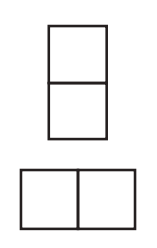
\includegraphics[width = 0.2\textwidth]{2dominoes.png}
    \end{center}
    \caption{8$\times$8 Checkerboard tiled with two dominoes}
\end{figure}
As we can see from \textbf{Figure 1}, all the squares on the checkerboard are filled with 32 two dominoes horizontally. Moreover, this is also a constructive existence proof that show we can use dominoes to tile rectangular checkerboard
with an even number of squares. Additionally, there are still many ways to tile a checkerboard
not only place it horizontally.
\subsection*{Exercise 46}
Prove or disprove that you can use dominoes to tile a 5 $\times$ 5 checkerboard with three corners removed.
\subsubsection*{Solution}
\clearpage
\begin{figure}
    \begin{center}
        
\includegraphics[width = 0.7\textwidth]{5x5Checkerboard-01.png}
    \end{center}
    \caption{5$\times$5 Checkerboard}
\end{figure}
As we can see from the 5$\times$5 checkerboard on \textbf{Figure 2}, there are 13 black squares
and 12 white squares. If we remove 3 black squares at three corner of the checkerboard,
there will be remain 10 black squares and 12 white squares. \\

From \textbf{Exercise 45}, we can tile the checkerboard with even squares but it requires that the number of white squares
and the number of black squares must be equal so that they can tile the checkerboard. For example,
the 8$\times$8 checkerboard has 64 squares so that there will be 32 black squares and 32 white squares.
However, in this Exercise, it remains 10 black squares and 12 white squares
so it has together 22 squares. 22 squares mean that there are 11 black squares
and 11 white squares. This create a contradiction that the checkerboard only contains
10 black squares and 12 white squares but it requires 11 black squares and 11
white squares to tile the checkerboard. So we can infer that we can not tile the 5$\times$5
checkerboard with three corners removed.
\subsection*{Exercise 47}
Use a proof by exhaustion to show that a tiling using
dominoes of a 4 $\times$ 4 checkerboard with opposite corners
removed does not exist.
\subsubsection*{Solution}
\begin{figure}
    \begin{center}
        
\includegraphics{4x4CheckerBoard.jpeg}
        \caption{\(4 \times 4\) Checkerboard}
    \end{center}
\end{figure}
Firstly, assume that the squares in the upper left and lower right corners
removed. Number of the squares of the original checkerboard from 1 to 16,
starting in the first row, moving right in this row, then starting in the 
leftmost square in the second row and moving right, and so on. We will remove
squares 1 and 16.\\

To prove this by using proof by exhaustion, we will divide the problem into
2 cases:
\begin{itemize}
    \item The first dominoes is laid horizontally start from square 2. So the first dominoes
    will cover square 2-3. After that, the other squares covered by dominoes
    in this order: 4-8, 6-7, 5-9, 10-11, 13-14. Therefore, there are 2 square
    left that are not covered are squares 12 and 15. So this case is impossible.
    \item The first dominoes is laid vertically start from square 2. So the first dominoes
    will cover square 2-6. After that, the other squares covered by dominoes
    in this order: 3-4, 4-8, 5-9, 10-11, 13-14. Therefore, there are 2 square
    left that are not covered are squares 12 and 15. So this case is impossible.
\end{itemize}
Because two cases above are all possible so we can infer that a tiling using dominoes of a 4 × 4
checkerboard with opposite corners removed does not exist.
\subsection*{Exercise 48}
Prove that when a white square and a black square are removed from an 8 \(\times\) 8 checkerboard (colored as in the text) you can tile the remaining squares of the checker- board using dominoes.
\subsubsection*{Solution}
\begin{figure}
    \begin{center}
        \includegraphics*{8x8CheckerBoardBarrier.png}
        \caption{Checkerboard with barrier}
    \end{center}
\end{figure}
As we can see from the \textbf{Figure 4}, within the barrier the checkerboard
is become a 64 continuos squares on the checkerboard. It starts at the upper
 left corner, go all the way to the right, then all the way down, then all
  the way to the left, and then weave your way back up to the starting point.
Therefore, the checkerboard will start at white square and end at black square.
Moreover, this rule is \textbf{true} for every single path on the checkerboard
which has these barriers. If it starts with white and ends with black, these paths
can be tiled with dominoes. Moreover, because path starts with white and
end with black, therefore, its length will be an even number.\\

With the rule we established above, we can infer that if we remove one random 
white square and black square, it will break this 64 continuos squares path into
2 different path start with white square and end with black square(their length will
be an even number) and all two paths can be tiled with dominoes. There will be
2 examples below:
\clearpage
\begin{figure}
    \begin{center}
        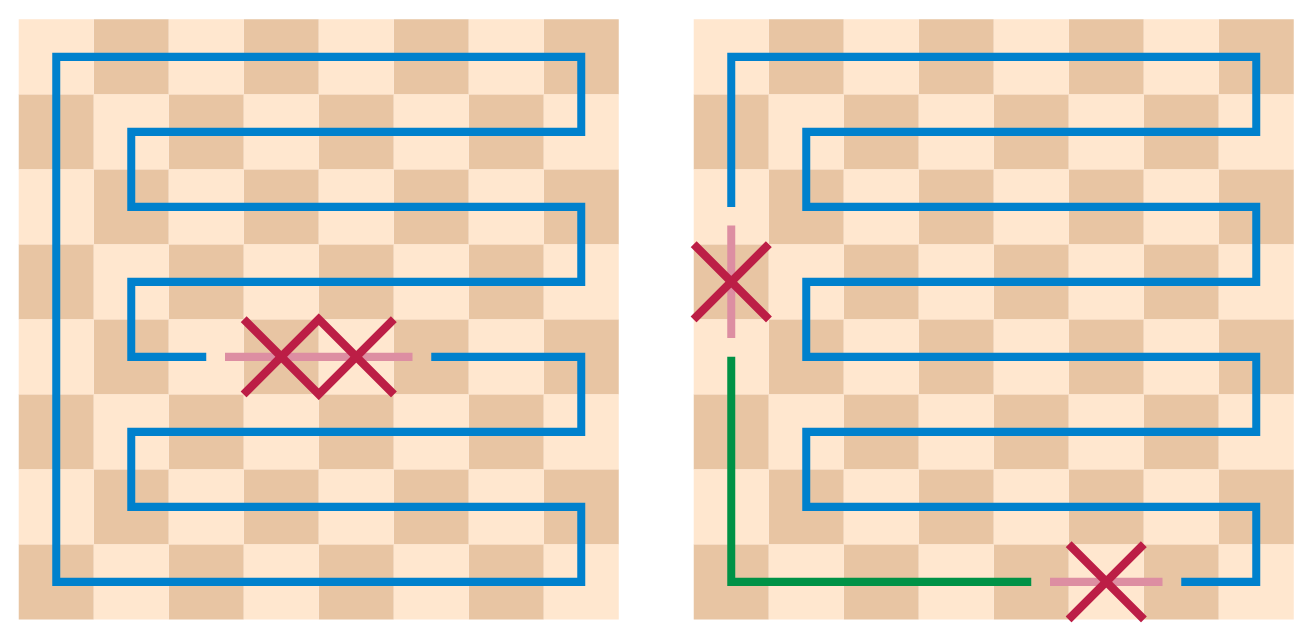
\includegraphics[width = 0.8\textwidth]{GomoryTheorem-01.png}
        \caption{Example of Exercise 48}
    \end{center}
\end{figure}
As you can see from \textbf{Figure 5}, if we remove two opposite color square,
we still can tile the whole checkerboard by tiling two paths created by 
removing two opposite color square with even length.
\subsection*{Exercise 49}
Show that by removing two white squares and two black squares from an 
8 \(\times\) 8 checkerboard (colored as in the text) you can make it 
impossible to tile the remaining squares using dominoes.
\subsubsection*{Solution}
\begin{center}
    
\begin{tikzpicture}[x=1cm]
        \foreach \y in {0,2,...,6}{
            \foreach \x in {0,2,...,6}{
                \fill (\x,\y) rectangle (1+\x,1+\y) rectangle (2+\x,2+\y);}}
    \end{tikzpicture}
\end{center}
So to prove that by removing two white squares and two black squares from an 
8 \(\times\) 8 checkerboard (colored as in the text) you can make it 
impossible to tile the remaining squares using dominoes, we will use existence
proof, which means that we just need to work out a example that can make
the 8 \(\times\) 8 checkerboard can not be tiled by removing two white squares and
two black squares. Therefore, we have an example:
\begin{itemize}
    \item WLOG, if we first remove two black squares which is adjacent to the white
    corner square. Next, we will continue remove to white squares which is adjecent to
    the black corner square. Therefore, there obviously impossible to tile that checkerboard
    because the domino can not cover two diagonal squares.
\end{itemize}
Because it exists a case that when we remove two black squares and two white square
from an 8 \(\times\) 8 checkerboard that make the checkerboard can not be tiled.
Therefore, we can prove that by removing two white squares and two black squares from an 
8 \(\times\) 8 checkerboard (colored as in the text) you can make it 
impossible to tile the remaining squares using dominoes.
\subsection*{Exercise 50}
Find all squares, if they exist, on an 8 \(\times\) 8 checkerboard such that 
the board obtained by removing one of these squares can be tiled using 
straight triominoes.
\clearpage
\subsubsection*{Solution}
\begin{figure}
    \begin{center}
        
\includegraphics[width = 0.8\textwidth]{8x8Checkerboard3Color.png}
        \caption{8 \(\times\) 8 checkerboard with 3 colors}
    \end{center}
\end{figure}
As we can see from \textbf{Figure 6}, there are 21 black squares, 21 blue squares
and 22 white squares (64 total). Next, we will check about three cases for the
removed square. When we remove one square, there will be 63 squares left:
\begin{itemize}
    \item The square removed is black square:\\ 
    If we remove one black square, there will be 20 black, 21 blue and 22 white left.
    However 63/3 = 21, which means that there will be 21 black, 21 blue and 21 white 
    but we only have 20 black, 21 blue and 22 white so it is a contradiction.
    Therefore, this case is impossible.
    \item The square removed is blue square:
    If we remove one blue square, there will be 21 black, 20 blue and 22 white left.
    However 63/3 = 21, which means that there will be 21 black, 21 blue and 21 white 
    but we only have 21 black, 20 blue and 22 white so it is a contradiction.
    Therefore, this case is impossible
    \item The square removed is white square:
    If we remove one white square, there will be 21 black, 21 blue and 21 white left.
    Moreover, 63/3 = 21 so there will be exist a checkerboard with one white square
    removed can be tiled using string triominoes. Additionally, we can also see that
    on the checkerboard, the coordinate (3,3), (3,6), (6,3), (6,6) is always keep
    white color no matter we rotate the checkerboard. Because only these four squares
    keep the color in all condition so that if we remove on of these square, we are able
    to tile the checkerboard within one square missing.\\

    As we can see from \textbf{Figure 7}, the coordinate (3, 3) square is the only
    square which is not filled by triominoes so if we remove this square and so on the 3 other
    coordinates above. Therefore, it exist the board can be tiled with one square removed.
\end{itemize}
\begin{figure}
    \begin{center}
        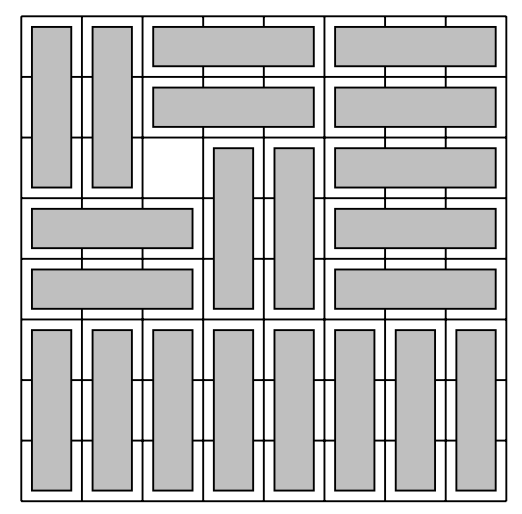
\includegraphics{8x8CheckerboardTri.png}
        \caption{8$ \times $8 checkerboard with one white square removed}
    \end{center}
\end{figure}
\subsection*{Exercise 51}
\begin{enumerate} [label = (\alph*)]
    \item Draw each of the five different tetrominoes, where a tetromino is a polyomino consisting of four squares.
    \item For each of the five different tetrominoes, prove or disprove that you can tile a standard checkerboard using these tetrominoes.
\end{enumerate}
\clearpage
\subsubsection*{Solution}
\begin{enumerate} [label = (\alph*)]
    \item We will have five different tetrominoes in \textbf{Figure 8}
    \begin{figure}
        \begin{center}
            \includegraphics*{5dominoes.png}
            \caption{Five different tetrominoes}
        \end{center}
    \end{figure}
    \item Now we will divide into 5 cases to check if all of these
    tetrominoes can tile a standard $ 8 \times 8 $ Checkerboard.
    \begin{itemize}
        \item The first tetrominoes is the same as two dominoes stand next
        to each other. Therefore, instead of using 32 dominoes to tile
        a checkerboard, we just need to use 16 tetrominoes(1).
        \item The second tetrominoes is the same also the same as
        two dominoes connect vertically. Therefore, instead of using
        32 dominoes to tile a checkerboard, we just need to use 16 tetrominoes(b).
        \item In this third tetrominoes, we will need to have one more symmetry one
        of this third tetrominoes, and then upside down the symmetry one and connect
        two of them, it will create a tetrominoes(2) with two columns. Thus,
        we can tile a checkerboard with 16 tetrominoes(2).
        \item In this fourth tetrominoes, if we connect 4 tetrominoes(3)
        with correct order, you will create a $ 4 \times 4 $ square(see in the \textbf{Figure 9} below).
        With this $ 4 \times 4 $ square, we can easily tile a standard checkerboard.
        \item In this fifth tetrominoes, we will label the squares of the checkerboard.
        Start from the upper left corner is 1 and go from left to right for each row.
        Therefore, the lower right corner of the checkerboard will be 64.\\ 
        We can see that if we put the tetrominoes on the upper left corner, it will
        cover square 1-2-10-11. Continue this process by putting the next tetrominoes horizontally
        to the first tetrominoes. Consequently, it will have the order of square covered:
        3-4-12-13,5-6-13-14. Thus, there are still squares 7 and 8 on the checkerboard can not be tiled with
        the shape of fifth tetrominoes. Therefore, it we can not tile the checkerboard with using tetrominoes(5).
    \end{itemize}
    \begin{figure}
        \begin{center}
            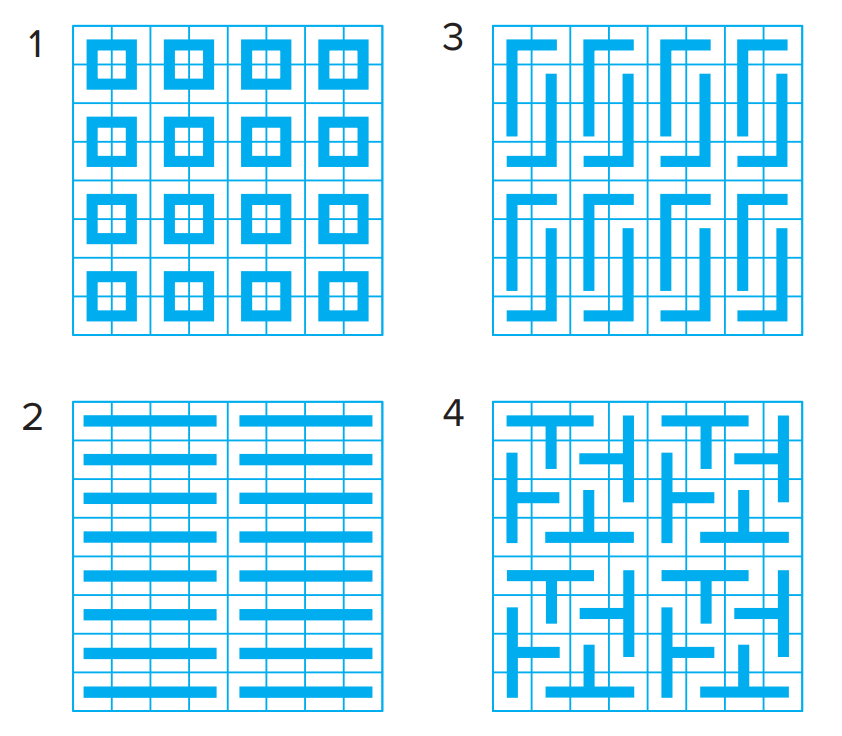
\includegraphics[width = 0.8\textwidth]{CheckerTileWith4Cases.png}
            \caption{Standard checkerboard tiled with 4 different tetrominoes}
        \end{center}
    \end{figure}
\end{enumerate}
\clearpage
\subsection*{Exercise 52}
Prove or disprove that you can tile a 10 $ \times $ 10 checkerboard using straight tetrominoes.
\subsubsection*{Solution}
In this exercise, we will label each four squares continuos 4 different colours 
white, black, blue, yellow respectively. Therefore, there will be 26 white squares,
26 black squares, 24 blue squares, 24 yellow squares. However, if we use
a straight tetrominoes for $ 10 \times 10 $ checkerboard, it is 100/4 = 25, which means that 
it will be 25 squares for each square but at we see that the checkerboard
has 26 white, 26 black, 24 blue, 24 yellow. Therefore, it creates a contradiction between the number
of each color. So that we cannot tile a 10 $\times$ 10 checkerboard with straight tetrominoes.
\begin{center}
    \textbf{THE END}
\end{center}
\end{document}